% !TeX root = ../main.tex

\chapter{Background}
\label{chapter:background}

\section{Isabelle}
\label{section:isabelle}
\emph{Isabelle} is a generic interactive theorem prover, which is mostly used for higher-order logic. \citeauthor{lpi} introduced Isabelle in 1986~\parencite{lpi}, the project is now being maintained and further developed by the Technical University of Munich, the University of Cambridge and countless independent contributors, the most active contributor being Makarius Wenzel. Isabelle, itself, is programmed and can be extended in Standard ML and Scala. A considerable number of theorems from mathematics and computer science have been formalized in Isabelle, many of which are stored in the \emph{Archive of Formal Proofs}. As of 2021, the Archive of Formal Proofs contains 602 Articles from almost 400 Authors~\parencite{afp}.

\subsection*{Isabelle/Isar}
\emph{Isar} (Intelligible semi-automated reasoning) is the formal proof language offered by Isabelle. It is inspired by the \emph{Mizar} system. Unlike Mizar, Isar is immediately 'executable', through the Isar/VM interpreter. Interactive theory and proof development is directly supported in Isar. It makes possible writing naturally understandable proofs, although this does take skill and effort from the writer~\parencite{isar_ref}.

\subsection*{Isabelle/Scala}
\emph{Scala} is a statically typed programming language~\parencite{scala} and it is used to develop the systems around the Isabelle environment. It enables services and systems from outside to access Isabelle. \emph{PIDE} (Prover IDE) is one of the most important services based on Isabelle/Scala and it is Isabelle's general framework for Prover IDEs. It works as a back-end for different source code editors and IDEs, by asynchronously processing source documents and providing support for editing, markup and other language features. The document model is central to the PIDE architecture, with source files being managed by PIDE and the physical file-system only playing a subordinate role~\parencite{isabelle_jedit}.

\subsection*{Isabelle/jEdit}
\emph{Isabelle/jEdit} is the main front-end of Isabelle/PIDE. It is based on the original \emph{jEdit}, which is an open source "programmer's text editor" written in Java~\parencite{jedit}. jEdit can be extended by plugins written in languages that run on the \emph{JVM}. %jEdit maintains a buffer for each file, with each buffer being associated to any number of visible text areas. Buffers are subject to an edit mode, which is determined from the file name or the file name extension.
Isabelle/jEdit is a slightly modified version of jEdit with an added plugin for Isabelle. Most of the language features, which are common in modern code editors, are supported by Isabelle/jEdit for Isabelle specifically. In Isabelle/jEdit the following language edit modes are supported, as shown in \autoref{fig:jedit_modes}:

\begin{table}[ht]
  \centering
  \begin{tabular}{l l l}
    \toprule
        edit mode & file name & content \\
    \midrule
        isabelle & *.thy & Theory source \\
        isabelle-ml & *.ML & Isabelle/ML source \\
        sml & *.sml or *.sig & Standard ML source \\
        isabelle-root & ROOT & Isabelle session root \\
        isabelle-options & & Isabelle options \\
        isabelle-news & & Isabelle NEWS \\
    \bottomrule
  \end{tabular}
  \caption{Language edit modes supported in Isabelle/jEdit~\parencite{jedit}.}
  \label{fig:jedit_modes}
\end{table}

\section{VSCode and VSCode Extensions}
\label{section:vscode}
\emph{VSCode} is a source-code editor developed by Microsoft~\parencite{vscode}. It is a commercial distribution of the open source project \emph{Code - OSS} which is also developed and maintained by Microsoft~\parencite{code_oss}. Since its initial release in April 2015, VSCode has managed to gain a great deal of popularity amongst developers, as illustrated in \autoref{fig:editors_pop}.

\begin{figure}[ht]
    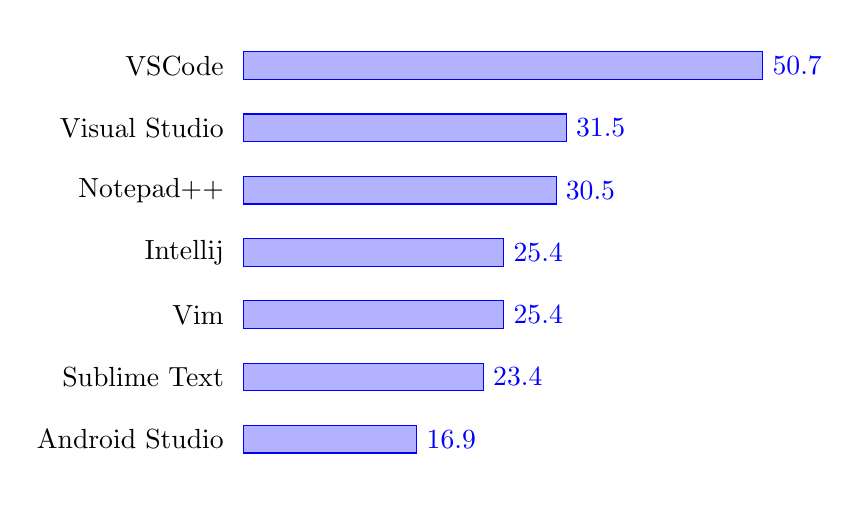
\begin{tikzpicture}
      \begin{axis}[
        xbar,
        y axis line style = { opacity = 0 },
        axis x line       = none,
        tickwidth         = 0pt,
        ytick = data,
        enlarge x limits  = 0.02,
        symbolic y coords = {Android Studio, Sublime Text, Vim,Intellij, Notepad++,Visual Studio,  VSCode  },
        nodes near coords,
        xmin= 0, %
      ]
      \addplot coordinates { (16.9,Android Studio) (50.7,VSCode)         (31.5,Visual Studio) (30.5,Notepad++)  (25.4,Intellij) (25.4,Vim) (23.4,Sublime Text)  };
    \end{axis}
    \end{tikzpicture}
    \caption{Percentage of developers who use the editor, 2019 survey~\parencite{editors_pop}.}
    \label{fig:editors_pop}
\end{figure}

VSCode is based on the \emph{Electron} framework, which makes it easy to be ported in multiple platforms. Because it is an Electron based application, VSCode makes use of mainly web technologies.

VSCode functionality can be added via extensions, which can either be published to the VSCode Extension Marketplace or be packaged into the VSIX format and shared with other users. To develop extensions VSCode offers its \emph{Extension API}~\parencite{extension_api}, which is fairly powerful for most use cases. Many core features of VSCode are built as extensions and use the same Extension API, for example the default git integration~\parencite{git_integration}.

Extensions can be developed with \emph{TypeScript} or \emph{JavaScript}. TypeScript being the preferred language, since most of the guides and examples are written in TypeScript. For packaging, publishing and managing extensions, VSCode offers its own command-line tool "vsce" (short for Visual Studio Code Extensions), available on \emph{npm}~\parencite{vsce_npm}.

In VSCode, support for programmatic language features (i.e. auto completion, error checking, jump to definition, etc) is provided through the \emph{Language Server Protocol}.

\section{Language Server Protocol}
The Language Server Protocol was originally developed from Microsoft in collaboration with Red Hat and CodeEnvy specifically for VSCode. Now it is an open standard supported by many code editors.

Modern source code editors and IDEs support a wide range of sophisticated programmatic language features. Compilers and interpreters normally cannot provide these language features, since they are meant to work with well-formed source code. Language Servers are specifically developed to deal with these issues. They evaluate the syntactic and semantic outcomes from source code modifications and give instant feedback to the user.

Microsoft developed the Language Server Protocol to solve three common issues with Language Servers~\parencite{lsp_guide}.

\begin{enumerate}
    \item Language Servers are usually implemented in their native programming languages, and that presents a challenge in integrating them with VSCode, which has a Node.js runtime.

    \item Language Servers can be resource intensive. For example, to correctly validate a file, a Language Server may need to parse a large amount of files, build up Abstract Syntax Trees for them and perform static program analysis. Those operations could incur significant CPU/memory usage and VSCode's performance must remain unaffected.

    \item Integrating multiple language servers with multiple code editors could involve significant effort. This makes implementing language support for M languages in N code editors the work of M * N.
\end{enumerate}

\begin{figure}[ht]
    \centering
    \includegraphics[width=0.8\textwidth]{figures/background/multi-editor.png}
    \caption{Diagram showcasing how a language server interacts with multiple editors~\parencite{extensions_overview}.}
    \label{fig:lsp_example}
\end{figure}

By standardizing the communication between a Language Server and a Language Client (source code editors/IDEs), the Language Server Protocol allows one Language Server to be reused in multiple editors. \autoref{fig:lsp_example} is an illustration of how this works.

The language server protocol defines a set of JSON-RPC request, response and notification messages which are exchanged. The base protocol consists of a header and a content part (comparable to HTTP). The header and content part are separated by a \texttt{\textbackslash r\textbackslash n}. The only supported header fields are \emph{Content-Length} and \emph{Content-Type}. The header is encoded using the ASCII encoding, while the content part is encoded in UTF-8. The base protocol uses a convention such that the parameters passed to request/notification messages should be of object type (if passed at all). Every processed request must send a response back to the sender of the request. If a request doesn’t provide a value, the receiver of a request still needs to return a response message to conform to the JSON-RPC specification. A processed notification message must not send a response back~\parencite{lsp_spec}.

The protocol currently assumes that one server instance serves one tool. There is currently no support in the protocol to share one server between different tools. Such a sharing would require additional protocol e.g. to lock a document to support concurrent editing.


\section{Isabelle/VSCode}
The rising popularity of VSCode also caught the attention of the prover community. Theorem provers such as \emph{Coq}~\parencite{coq} and \emph{Lean}~\parencite{lean} started supporting their own extensions for VSCode, namely \emph{VSCoq}~\parencite{vscoq} and \emph{vscode-lean}~\parencite{vscode-lean}, as early as 2016. The Isabelle project shortly followed suit, with \citeauthor{ivsc_report} developing Isabelle/VSCode~\parencite{ivsc_report}.

The Isabelle/VSCode project consists of its VSCode extension and its server, which is instantiated through the Isabelle command-line tool. The extension and server communicate as specified by the Language Server Protocol, with some additional features/endpoints to support the idiosyncrasies of Isabelle and VSCode.

The server is an application written in Isabelle/Scala, with most of the functionality used directly from Isabelle/PIDE, but adapted to the Language Server Protocol endpoints. Communication between the client and the server happen mostly through notifications, aside from some a few endpoints which are explicitly set by the language server protocol as request/response endpoints.

%The main goal of the Isabelle/VSCode project is to achieve feature parity between it and Isabelle/jEdit. 